\chapter{Future directions}
\label{c:conclusion}

\section{Quantum feedback control}

The stabilization of Rabi oscillations was successful partially due to the simplicity of the direct feedback control law, which does not require complex signal processing to implement.  The extra delay time associated with real-time calculations, even in fast, dedicated digital hardware, is on the same order as the total analog loop delay measured in section \ref{s:loop_delay}, and this delay time played a large role in limiting the feedback performance.  With coherence times of superconducting qubits continually improving, the critical rates necessary to achieve good feedback performance can be relaxed as the qubit decoherence rates decrease.

With more dwell time available for signal processing calibrations, far more elaborate feedback protocols may be implemented.  For example, in the cavity QED experiment which demonstrated the stabilization of Fock states using feedback \cite{haroche_fb}, the coherence times of the Fock states were on the order of milliseconds, with one measurement Rydberg atom detected every 82 $\mu$s.  These time scales are long enough that a real-time computer was employed to use a complex Bayesian inference procedure to update a real-time estimate of the density matrix of the cavity state and apply a brief correction pulse.  This procedure included the effects of many experimental imperfections, including a relatively low atom detection efficiency of 35\% and the fact that the atom source sometimes failed to emit an atom.  As such, in spite of these inefficiencies, the feedback loop prepares the target state with a fidelity of about 0.8, and is able to rapidly detect a quantum jump in the field after only about 3 atom passages and begin applying a correction.

The other major limiting factor in the Rabi stabilization experiment was the relatively low quantum measurement efficiency achieved of at best 40\%.  By reducing the losses between the cavity and parametric amplifier this number can be improved somewhat, though typical system quantum efficiencies at QNL are still about 50\%.  Because the JTWPA does not intrinsically require a microwave circulator between the cavity and amplifier, it is possible that careful microwave engineering will permit the direct integration of the amplifier on the same chip as the qubit and cavity.  By eliminating the insertion loss associated with the intermediate microwave components, and with a modestly higher capacitor dielectric quality factor (readily achievable in other fabrication processes), the quantum efficiency of this setup could potentially read 80\%-90\%.

\begin{figure*}
\begin{center}
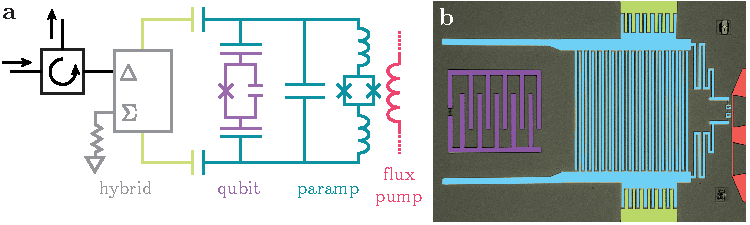
\includegraphics[width=5in]{conclusion/transamp}
\end{center}
\caption[Circuit model and chip photo of transamp]{\textbf{a} Circuit model of transamp, showing differential launch using hybrid, single-junction transmon qubit in purple, nonlinear resonator (LJPA) in blue, and the bias line used to flux-pump the LJPA (red).  \textbf{b} False-color electron-microscope image of a transamp chip; the coloring corresponds to the circuit schematic in \textbf{a}.}
\label{fig:transamp}
\end{figure*}
Another route to achieving high quantum efficiency is integrating the quantum-limited amplifier into the readout cavity itself.  There is an effort at QNL to do just this.  The device is called the \textit{transamp} (short for \textit{transmon amplifier}); a circuit schematic and an image of a fabricated device are shown in Figure \ref{fig:transamp}.  The basis for the transamp is to couple the transmon qubit directly to a nonlinear resonator, which is driven by a strong flux modulation.  This can be thought of as a dispersive circuit QED readout with some intrinsic gain at the level of the cavity itself.  Because of this gain, the losses between this device and the next following amplifier should not participate as strongly as they do in a normal cQED with following paramp setup.  The back-action of this type of readout is not as simple as the straightforward dispersive cQED readout, however, and achieving quantum-limited performance in this system is an outstanding experimental challenge.

A variety of interesting feedback protocols become possible in superconducting qubits with the addition of fast real-time signal processing, further improvements to the quantum measurement efficiency, or both.  Some examples of single-qubit experiments which would be possible with higher measurement efficiency include the rapid purification of an unknown qubit state using adaptive measurements \cite{PhysRevA.67.030301}, the potential demonstration of measurement-induced steering of the qubit state evolution during measurement \cite{PhysRevLett.108.220402}, and feedback control based purely on the quantum Zeno effect \cite{1367-2630-12-4-043005}.

Two similar experiments to the Rabi stabilization experiment have since been performed by other groups, utilizing fast digital electronics to implement more complex control protocols.  In reference \cite{DeLange2014}, an FPGA was used as the feedback controller to enable the stabilization of the qubit along the $x$-axis of the Bloch sphere with an efficiency of about 50\%, limited by the quantum measurement efficiency.  In reference \cite{campagne-ibarcq_persistent_2013}, Rabi oscillations were stabilized using stroboscopic projective measurements to check the state of the qubit during the moments of the oscillation corresponding to qubit eigenstates.  A fast control protocol implemented in an FPGA applied a $\pi$-pulse to flip the qubit state if it was not found in the right state.  The reliance on projective measurements relaxes the stringent requirement on quantum efficiency, allowing a stabilization of Rabi oscillations with a fidelity of 85\%.

The remote entanglement-by-measurement experiment performed at QNL \cite{Roch2014} only created two-qubit entanglement in a probabilistic manner.  Adding feedback control to this experiment could enable the deterministic creation of this entanglement by actively driving the system back into the entangled state when the continuous joint measurement detects evolution towards an error state \cite{Sarovar:2005kx,PhysRevLett.111.170404}.  A version of this experiment utilizing projective measurements on the joint state of two qubits in the same cavity has been experimentally demonstrated in reference \cite{Riste2013}.

\section{JTWPA development}

Although the JTWPA device discussed in chapter \ref{c:twpa_exp} is the result of several years of development, it is essentially still a first-generation device.  Now that the theory has been validated, and a working device demonstrated, there is plenty of engineering left to do to create a more highly optimized device.

The dynamic range of the JTWPA is essentially set by the junction critical current.  From the discussion in section \ref{s:twpa_param}, if we were to increase the dynamic range by raising the junction critical current, the unit cell inductance and thus the gain would fall.  A similar constraint limits the dynamic range of JPAs, due to the relationship between bandwidth, center frequency, and critical current discussed in section \ref{s:jpa_perf}.  There is a technique which has been utilized in JPAs to sidestep this issue \cite{Eichler2014a}, which is to replace the single junction of critical current $I_0$ (and corresponding Josephson inductance $L \propto 1/I_0$) with a series array of $N$ junctions, each with critical current $NI_0$ (and inductance $L' = L/N$).  The total critical current of the array is then $N$ times larger, though the inductance has remained constant, enabling an increase in the maximum pump power of a factor of $N^2$.  Because of the need to utilize SQUIDs rather than single junctions to tune the center frequency of the amplifier, this technique cannot be pushed to an arbitrarily long array without eventually introducing instabilities related to multiple SQUID energy configurations.

This technique can be readily adapted to the JTWPA, and the picture is even more simple due to the fact that only junction arrays rather than SQUID arrays are necessary due to the large intrinsic bandwidth.  By moving towards mini-arrays of 3 junctions per unit cell, the dynamic range of the JTWPA could be increased by an order of magnitude.  This is a very minor design change, and should not increase the size of the device as the junctions are by far the smallest circuit element.  It is not presently understood if this approach has any fundamental limitations; a move to 10-junction mini-arrays in each unit cell would push the dynamic range up by two orders of magnitude.  Based on the extrapolation in section \ref{s:twpa_proj_meas}, such a large dynamic range is not necessary for the readout of, say, 100 qubits (and, moreover, the resource overhead of adding another quantum-limited amplifier is small compared to the resource overhead of dozens of qubits), so scalable quantum computing may not be an application that demands pushing this approach to the limit.

The gain profile of the JTWPA shown in section \ref{s:gain_with_rpm} is not completely smooth, but contains some $\sim 2$ dB ripples due to the imperfect impedance matching between the nonlinear transmission line and the linear feedlines.  This can be improved in future devices by more carefully matching the nonlinear impedance to 50 $\Omega$.  Some of this mismatch is also likely due to the wirebonds which make the connection between the chip and the PCB on which it is mounted.  Future JTWPA devices may be integrated directly on the same chip as the qubit and cavity, removing the need for the large CPW taper structure and the wirebonds.  This may further improve the impedance matching and reduce the gain ripple.

At present, an external directional coupler is used to inject the strong pump tone which drives the JTWPA.  This component introduces some loss, which reduces the overall quantum efficiency by about 0.5 to 1 dB.  Utilizing either a PCB-level or on-chip superconducting directional coupler, this component could be eliminated, reducing the total component count and eliminating some loss.  Alternatively, because the pump tone is narrowband and fixed in frequency to be near the RPM dispersion feature, a more specialized structure than a traditional directional coupler could be employed instead, as only narrowband directivity is required to isolate the pump from the amplifier's input port.

The layout of the JTWPA is reminiscent of a standard meandered transmission line with smooth bends.  However, the need for these features in a geometric transmission line fundamentally arises from the fact that the geometry of the transmission line sets the impedance, so smooth features are necessary to realize a consistent impedance.  In the JTWPA, the impedance is entirely set by the ratio of the size of the Josephson inductance to the capacitance to ground in each unit cell.  Because each unit cell is much shorter than a wavelength, only the electrical properties on the length scale of many tens of unit cells is important to wave propagation.  Thus, the smooth bends in the JTWPA could be eliminated in favor of sharp 90$^\circ$ corners.  Furthermore, because the transmission line inductance is almost entirely the kinetic inductance of the Josephson junction and the capacitance is formed from high-aspect-ratio, nearly-ideal parallel plate capacitors, the transmission line segments could be brought much closer together without any serious inter-trace coupling.  These two facts combined imply that the footprint of the JTWPA on chip could be \textit{significantly} reduced, quite possibly occupying an area an order of magnitude smaller than the present device.

Besides improvements in the engineering of the JTWPA, there remain plenty of fundamental science questions to be addressed in this system.  With no signal incident at the input of the JTWPA, the output state contains two-mode correlations at symmetrically detuned frequencies about the pump frequency.  If the quantum performance of the JTWPA turns out to be sufficiently ideal, these two-mode correlations should be large enough to realize two-mode squeezed states \cite{Loudon1987}.  These states have been generated using JPAs \cite{Eichler2011,PhysRevLett.108.123902} and have been utilized as a resource in quantum information processing \cite{PhysRevLett.114.090503}.  A technique has been proposed to utilize broadband two-mode squeezing to realize a high-fidelity projective qubit measurement on a much shorter time scale than what is possible using conventional cQED readout with unsqueezed light \cite{Didier2015}.  The JTWPA could be ideally suited to implementing this scheme, if future measurements of its squeezing properties reveal good performance.  A source of very broadband two-mode squeezing could also potentially enable future directions in microwave quantum optics which have not yet been imagined.



